\documentclass{beamer}
\usepackage{graphicx}
\usepackage{listings}
\usepackage{hyperref}

\usetheme{CambridgeUS}
\setbeamertemplate{navigation symbols}{}

\title{ReflectoRay: Ray Reflection Simulation}
\author{Team ReflectoRay}
\date{\today}

\begin{document}

\begin{frame}
  \titlepage
\end{frame}

\begin{frame}{Outline}
  \tableofcontents
\end{frame}

\section{Introduction}
\begin{frame}{Introduction}
  \begin{itemize}
    \item Developed by Team ReflectoRay
    \item Zewail City - University of Science and Technology
    \item Fall 2023
  \end{itemize}
\end{frame}

\begin{frame}{Team Members}
  \begin{itemize}
    \item 202201079 - SalahDin Ahmed Salh Rezk \\
          \href{mailto:s-salahdin.rezk@zewailcity.edu.eg}{s-salahdin.rezk@zewailcity.edu.eg}
    \item 202201293 - Ahmed Muhammad Abdullah \\
          \href{mailto:s-ahmed.abdullah@zewailcity.edu.eg}{s-ahmed.abdullah@zewailcity.edu.eg}
    \item 202201517 - Salah Mahmoud Gamal \\
          \href{mailto:s-salah.gamal@zewailcity.edu.eg}{s-salah.gamal@zewailcity.edu.eg}
  \end{itemize}
  \textbf{Team Contact:} \href{mailto:s-salahdin.rezk@zewailcity.edu.eg}{s-salahdin.rezk@zewailcity.edu.eg}
\end{frame}

\section{Problem Description}
\begin{frame}{Background}
  \begin{itemize}
    \item Understanding ray reflection in geometric optics
    \item Challenges in visualization and comprehension
  \end{itemize}
\end{frame}

\begin{frame}{Challenges}
  \begin{enumerate}
    \item Lack of Interactive Tools
    \item Difficulty in Visualization
    \item Configurability Limitations
  \end{enumerate}
\end{frame}

\begin{frame}{Project Rationale}
  \begin{itemize}
    \item Address challenges through ReflectoRay
    \item Python with Turtle graphics library
    \item Interactive and configurable platform
  \end{itemize}
\end{frame}

\section{Solution Description}
\begin{frame}{Key Features}
  \begin{itemize}
    \item Interactive Visualization
    \item Configurability
    \item Visualization Enhancements
    \item Image and Video Output
    \item Progress Visualization
  \end{itemize}
\end{frame}

\begin{frame}{Advantages}
  \begin{itemize}
    \item Enhanced Learning Experience
    \item Versatility
    \item Documentation and Sharing
    \item Real-time Feedback
  \end{itemize}
\end{frame}

\begin{frame}{Expected Outcomes}
  \begin{itemize}
    \item Educational tool for geometric optics
    \item Hands-on and engaging learning experience
    \item Configurable for different scenarios
    \item Image and video documentation
  \end{itemize}
\end{frame}

\section{Implementation Details}

\begin{frame}{System Requirements}
  \begin{itemize}
    \item Python 3.x installed
    \item Required Python libraries: Turtle, OpenCV, PIL, Rich
  \end{itemize}
\end{frame}

\begin{frame}{Installation}
  \begin{itemize}
    \item Install Python
    \item Install required libraries: \\
          \texttt{pip install turtle opencv-python pillow rich}
  \end{itemize}
\end{frame}

\begin{frame}{Running the Simulation}
  \begin{itemize}
    \item Clone the repository
    \item Navigate to the project directory
    \item Configure the simulation in \texttt{initial\_conditions.json}
    \item Run the simulation: \texttt{python reflectoray.py}
  \end{itemize}
\end{frame}

\begin{frame}{Save the Simulation}
  \begin{itemize}
    \item Save as image: \texttt{python reflectoray.py --image}
    \item Save as video: \texttt{python reflectoray.py --video}
  \end{itemize}
\end{frame}

\begin{frame}{Simulation Output}
  \begin{figure}
    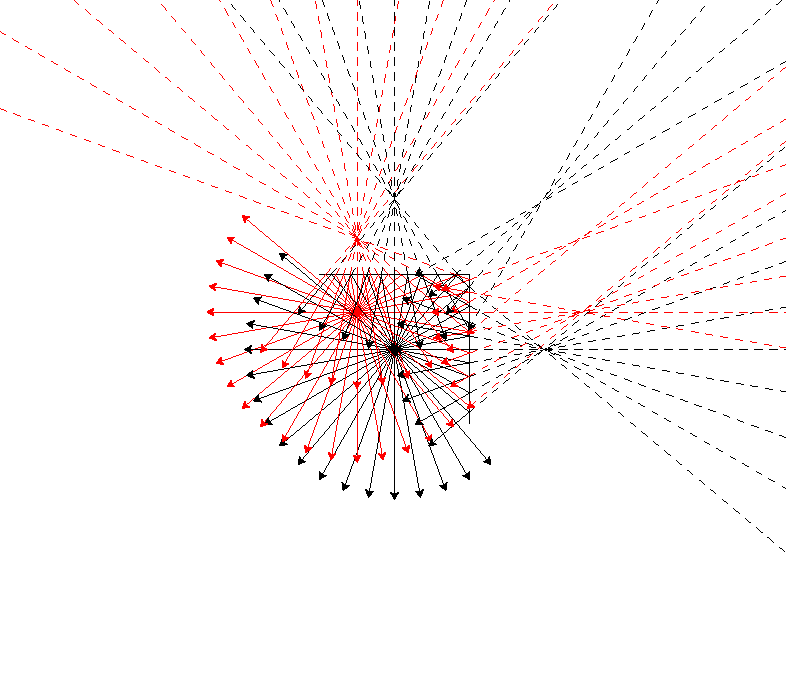
\includegraphics[width=0.8\textwidth]{figures/20231106-112653.png}
    \caption{Simulation Image Output (default initial conditions)}
  \end{figure}
\end{frame}

\end{document}
